% vim:ft=tex:
%
\documentclass[12pt]{memoir}
\usepackage[margin=1in]{geometry}
\usepackage{graphicx}

\begin{document}

\pagenumbering{gobble}

\begin{center}
  \textbf{Interaction Techniques and Active Learning Methods for Mixed Initiative Exploration of Fabrication Hardware Parameter Spaces}\\
  \vspace{.5em}
  Andrew Head
\end{center}

If you walk into the foyer of the Invention Lab, Berkeley's student hackerspace, you'll see dozens of failed 3D prints lined up around periphery of the entry way.
Talk to any of the students or the staff on hand and you'll find out:
\emph{Getting started with fabrication hardware is hard.}
What all goes wrong?
Well, a few different things.
3D printing without large enough tolerances leaves movable parts stationary.
Thin supports or sharp overhangs result in tangled spindles of ABS that fail to layer properly.
On the laser cutter, vector cutting with too much power can set the workpiece on fire from the deadly beam of energy powering through to the material.
With each new material and image they want to imprint, raster settings will have to be manipulated to the right power and speed to yield a setting that is both as deep as desired, but also that doesn't cause melting or charring, all at a quick enough pace to finish the workpiece fast enough to let others use the machine.

Reading through the guides on use of the machine can shed light into how to properly use the laser cutter:
there are four configurable parameters that will affect how the beam interacts with the material.
\emph{Power} controls the intensity of the beam, \emph{speed} modulates how quickly the laser moves over the material, \emph{frequency} determines the periodicity of the beam firing at the material, and \emph{resolution} determines how close ``pixels'' of a raster are placed to each other on the material.
The values of these are set to vary based on the material a user is working with, the speed they want to work to get done with, the depth of the marks, and how rough of a sketch they can accept for the current raster.
But a na\"{\i}ve user is unlikely to know how to set machine parameters for a new material, or to systematically vary these parameters until a raster.
A major failure occurs in that the hacker will likely want to use the machine long before they want to develop an accurate mental model of how the parameters impact the work to be done.

For fabrication hardware, there is a comically unsurmountable correspondence problem.
People do not have nozzles out of which they can extrude molten plastic, nor do they have laser beams that can be blasted to melt materials.
There is no clear way how learning from demonstration techniques can be used to describe configurations for settings such as laser power, speed, frequency, and resolution.
Furthermore, these parameters don't map directly to the task the user wants to perform.
The hacker may have a clear idea of the appearance of the material surface that they want to attain, and an understanding of how these parameters cause it just is not clear.

This work aims to answer the following questions that, to my knowledge, are open questions within both the fields of human-robot interaction and the fabrication concentration of human-computer interaction.
First, \textbf{how can a robot learn an ideal configuration for a task when no demonstration is given?}
Second, \textbf{what are the most efficient subjective inputs and interaction techniques to enable fast convergence to an ideal configuration with a fabrication machine?}

This study will begin with an observational study with student members of the Invention Lab (around $n=5$).
These students will be interviewed to better understand the frequency, severity, and types of errors students encounter expressing designs to fabrication hardware.
Questions will include:
What jobs have you submitted in the past that have failed?
How many times did you have to iterate on this artifact before it was successfully fabricated?
What did you learn about the capabilities of the hardware after this effort?

Then I will implement an active learning scheme~\cite{settles_active_2010} that will collect user ratings for raster jobs based on example configurations of power, speed, resolution and frequency for a laser cutter, with the aim of predicting user ratings with a minimum number of examples.
While active learning in typical contexts (see~\cite{settles_active_2010}) has been applied to learning linear decision boundaries for binary classification, we will draw upon past work that seeks to adapt active learning to predicting continuous values for examples (e.g.~\cite{sugiyama_active_2008}).
Currently, I suspect that a Gaussian kernel function or a quadratic curve will best express a user's perception of the quality of a configuration in actualizing their design.

I will conduct a study to determine what input methods will be most successful in helping a user converge to a desired rastering configuration.
The usability study will be run in the Invention Lab with the Universal Laser Systems VLS3.50 machine, for which I have already received clearance to run user studies.
Subjects will be provided with a work piece they are asked to replicate.
One experimenter will direct the VLS3.50 to perform one raster job with configuration examples derived from the algorithm described above remotely (so that it is opaque to the participant).
The participant will be asked to rate each example, providing a score that will be fed back into the active learning algorithm.
After every third example, the model show the participant a raster with the optimal score according to the model learned so far.
The raster will be considered `complete' if the user offers it the top score on the Likert scale.
Subjects will all be exposed to three input methods via a simple web interface that connects back to the active learner:
Likert-scale ratings of the most recent example, arrangement of rank of all seen examples so far, and trial and error (no active learning, but manual configuration of parameters only.)

Given the limits of the hardware available in the Invention Lab, this study will likely include around 4 testers altogether.
Measurements collected will include the time and iterations taken to perform the task, Likert scale ratings of user satisfaction, and qualitative feedback about strategies to achieve the ideal rastering.

\begin{figure}
  \centering
  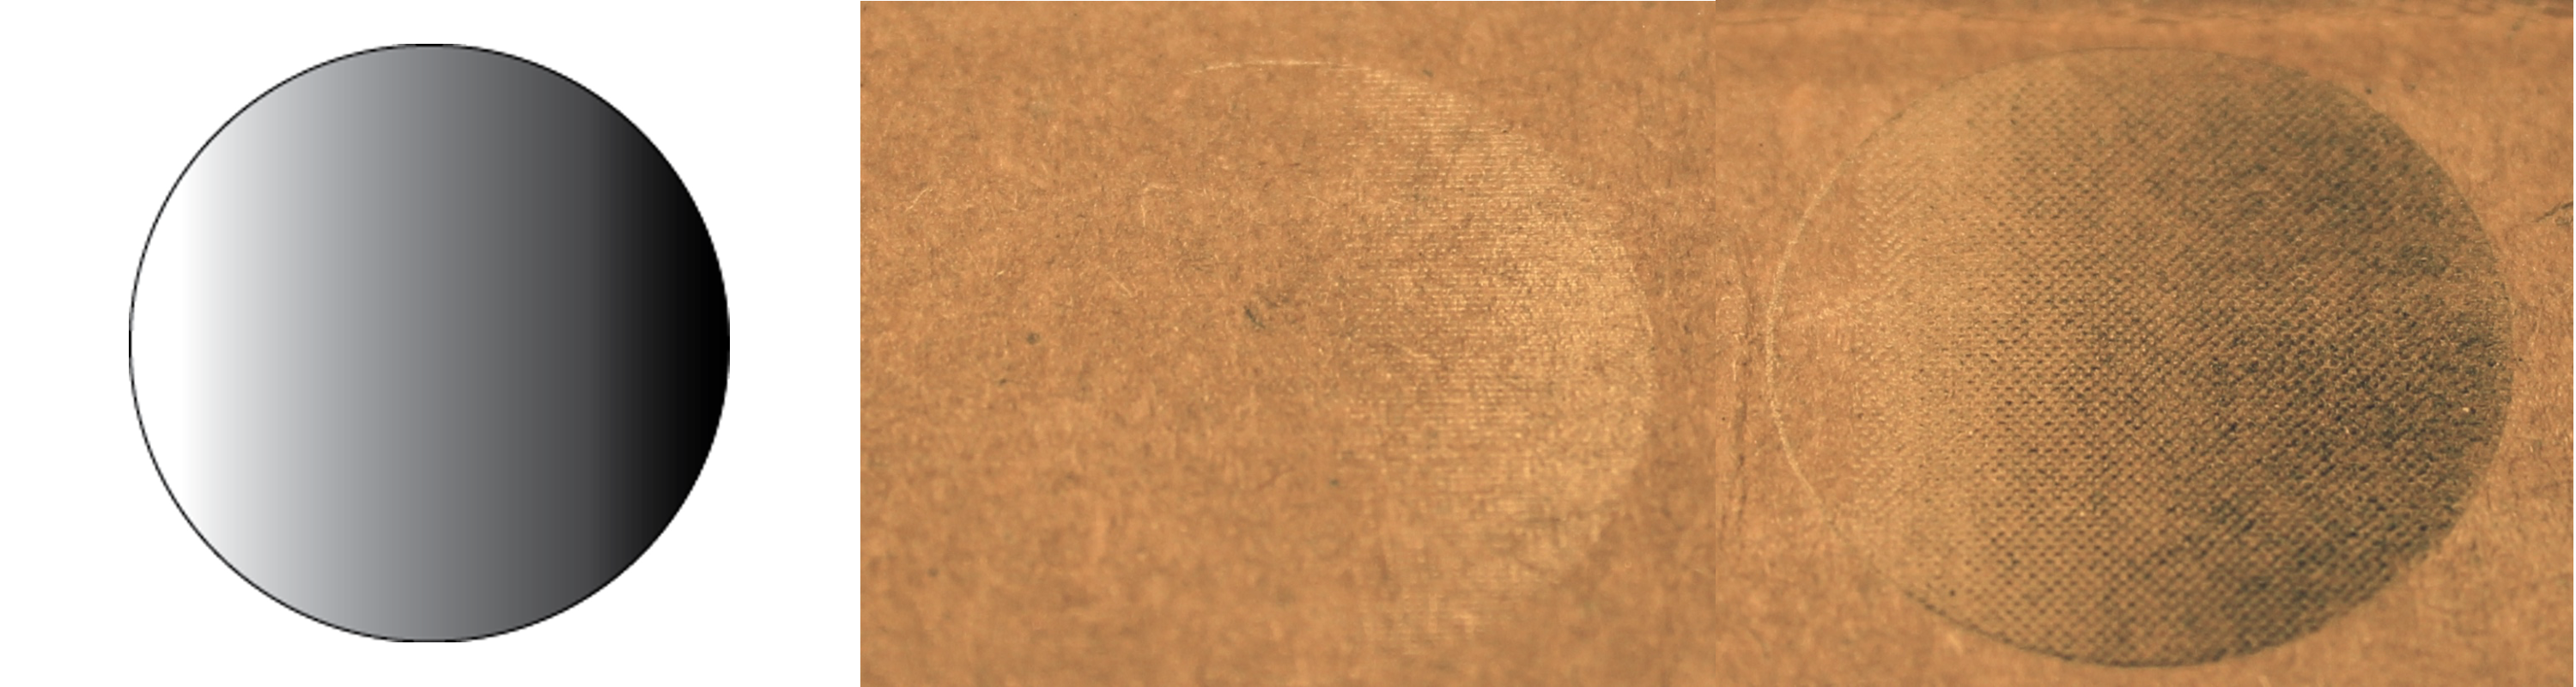
\includegraphics[width=0.6\textwidth]{figures/rasters}
  \caption{\scriptsize{%
  A drawing `rastered' into cardboard by a laser cutter with two different configurations.
  \emph{Left}: the original image given to the laser cutter.
  \emph{Center}: an etching that is too faint to see due to low power
  \emph{Right}: an etching that scorched the cardboard due to high power and low speed.
  A user of the laser cutter will have to manipulate the laser's parameters to get the desired appearance.}}
\label{fig:rasters}
\end{figure}

\end{document}
